\section{Communication Flow Diagram}

In this section the flow of communication within in the complete architecture (satellites and ground station) will be explained in detail.
\begin{figure}[ht]
\centering
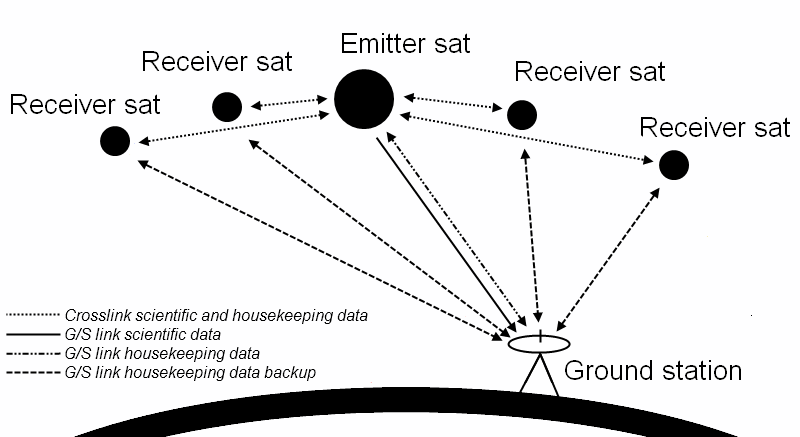
\includegraphics[width=1.0\textwidth, angle=0]{chapter/img/allesZW.png}
\caption{Complete communications architecture of the laser swarm}
\label{fig:allesZWW}
\end{figure}

Figure \cite{fig:allesZWW} shows all existing links and their place in architecture, with a legend in the lower left corner.
Three flows of communications exist in the architecture:
\begin{itemize}
\item Command data
\item Housekeeping data
\item Scientific data
\end{itemize}

Command data originates from the ground station, is transmitted to the emitter satellite over the G/S link for housekeeping and command data. In case the command data is required on a receiver satellite, the emitter satellite retransmits the data directly to that satellite over the crosslink for scientific, housekeeping and command data.

Housekeeping data flows in the exact reverse direction: the emitter satellite continuously receives the housekeeping data over the crosslinks from all the receiver satellites, then stores it and finally transmits it to the ground station together with its own housekeeping data over the G/S link for housekeeping data and command data.

In case the crosslinks are broken, command data and housekeeping data for and from the receiver satellites can still travel over the G/S link housekeeping and command data (backup).

The scientific data contains all the data on the registered photons (coordinates on the SPAD array, attitude and position of the satellites, timestamp). These are transmitted over the crosslinks to the emitter satellite, stored on its data storage system and then transmitted to the ground station over the G/S link for scientific data.
